\documentclass{article}
\usepackage{geometry, graphicx, float, subfigure, amsmath, bm}
\usepackage[marginal]{footmisc}
\geometry{a4paper,scale=0.8}

\title{\bf{pBR322 Mapping by Restriction Digestion with EcoR1/HincII/PvuII and Electrophoresis}}
\author{Xun Zhao (Partner: Samantha)}
\date{March 15, 2019}

\begin{document}
    \begin{titlepage}
        \maketitle
        \setcounter{page}{0}
        \thispagestyle{empty}
    \end{titlepage}

    \renewcommand{\abstractname}{Introduction}
    \begin{abstract}
        In order to defend the attack from virus, some bacterias can produce enzymes to digest invasive DNA molecule of virus. Among these kinds of enzymes, some of them cut DNA randomly, while others called restriction enzymes only cut at specific sequence. Thus, we can use these enzymes to digest the plasmid and get DNA fragments with different length. 

        As the cut sites are fixed in a plasmid, we can reconstruct the relative positions of restriction sites of a plasmid, called mapping.

        Firstly, we digest the plasmid with all possible combinations of 3 restriction enzymes. Then, we can use the agarose gel and certain voltage to separate negatively charged DNA fragments and use loading dye to indicate their positions under UV. And their travel distances are proportional to the reciprocal of logarithm of the number of base pairs, namely, the size of molecule compared with the size of holes in gel, which allows us to draw a standard curve from a reference plasmid with known structure. Finally, we can get the length from travel distance based on the standard curve and use these length to rebuild a plasmid.
    \end{abstract}

    \section{Results}
        \subsection{Raw Result Photo}
            To make the photo more readable, I convert\footnote{All the picture analysis below is based on the \textit{Fiji ImageJ}, including color converting and distance measuring.}
            the photo to black-and-white, adjust the contrast and label 9 wells.
            \begin{figure}[H]
                \centering
                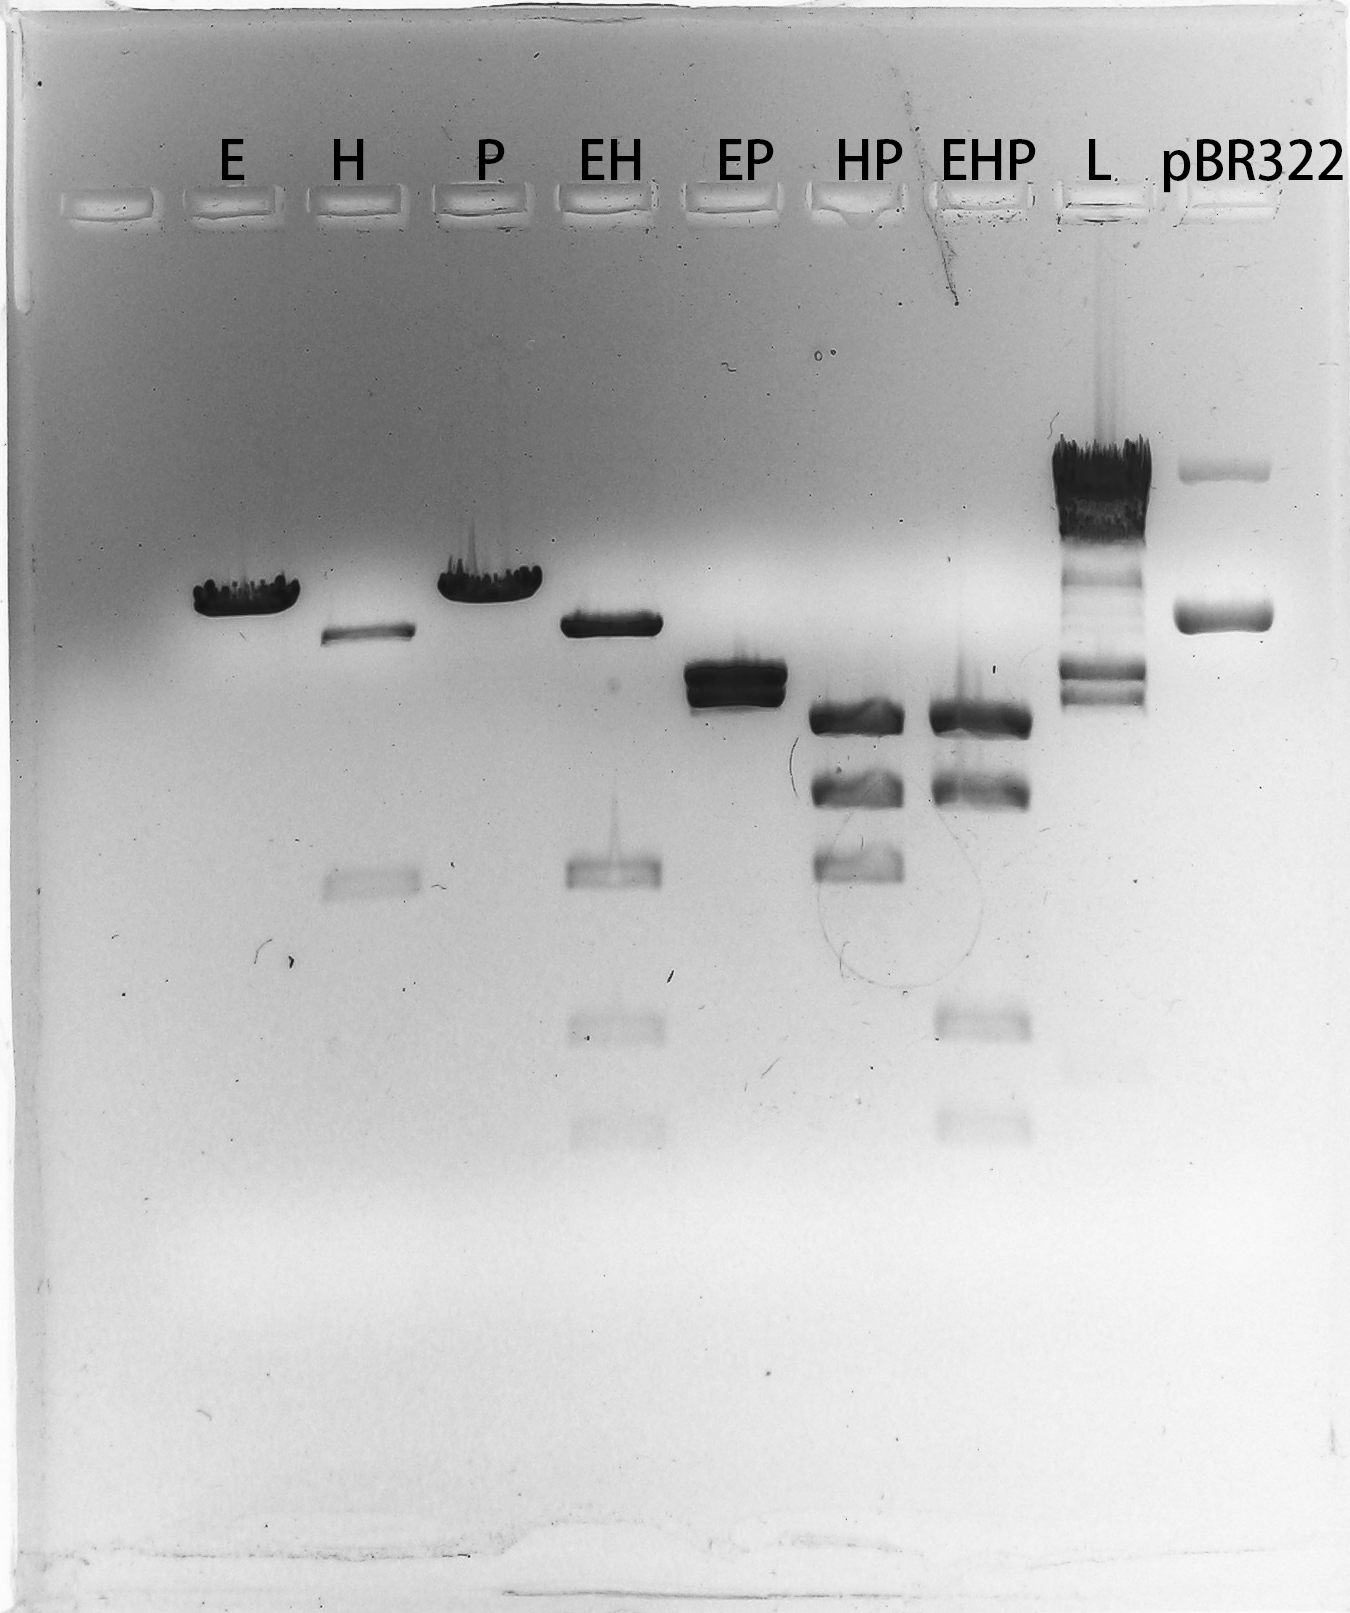
\includegraphics[width = 0.5\textwidth]{../Data/xun_and_sam.png}
                \caption{Raw Gel Photo}
            \end{figure}

        \subsection{\boldmath$\lambda\ $\unboldmath DNA data}
            Here is the known information of $\lambda$ DNA's fragments bands digested by \textbf{HindIII}, which is the $8^{\text{th}}$ well in the photo named {\bf{L}}.

            \begin{table}[H]
                \caption{$\lambda\ $DNA Data}
                \begin{center}\begin{tabular}{|l|c|c|r|}
                    \hline
                    &base pairs&log(bps)&distance (pixels)\\
                    \hline
                    1&      23130&4.364175633&266\\
                    2&      9461&3.97386645&292\\
                    3&      6557&3.816705184&326\\
                    4&      4361&3.639586087&376\\
                    5&      2322&3.365862215&468\\
                    6&      2027&3.306853749&502\\
                    7&      564&2.751279104&870\\
                    \hline
                \end{tabular}\end{center}
                \label{l.data}
            \end{table}

        \subsection{Standard Curve}

            We can write distance in terms of $d$, and base pairs in terms of $n$. According to the relationship, we will have,

            $$d \propto \frac{1}{log(n)}$$

            The raw curve is plotted as follows,
            \begin{figure}[H]
                \centering
                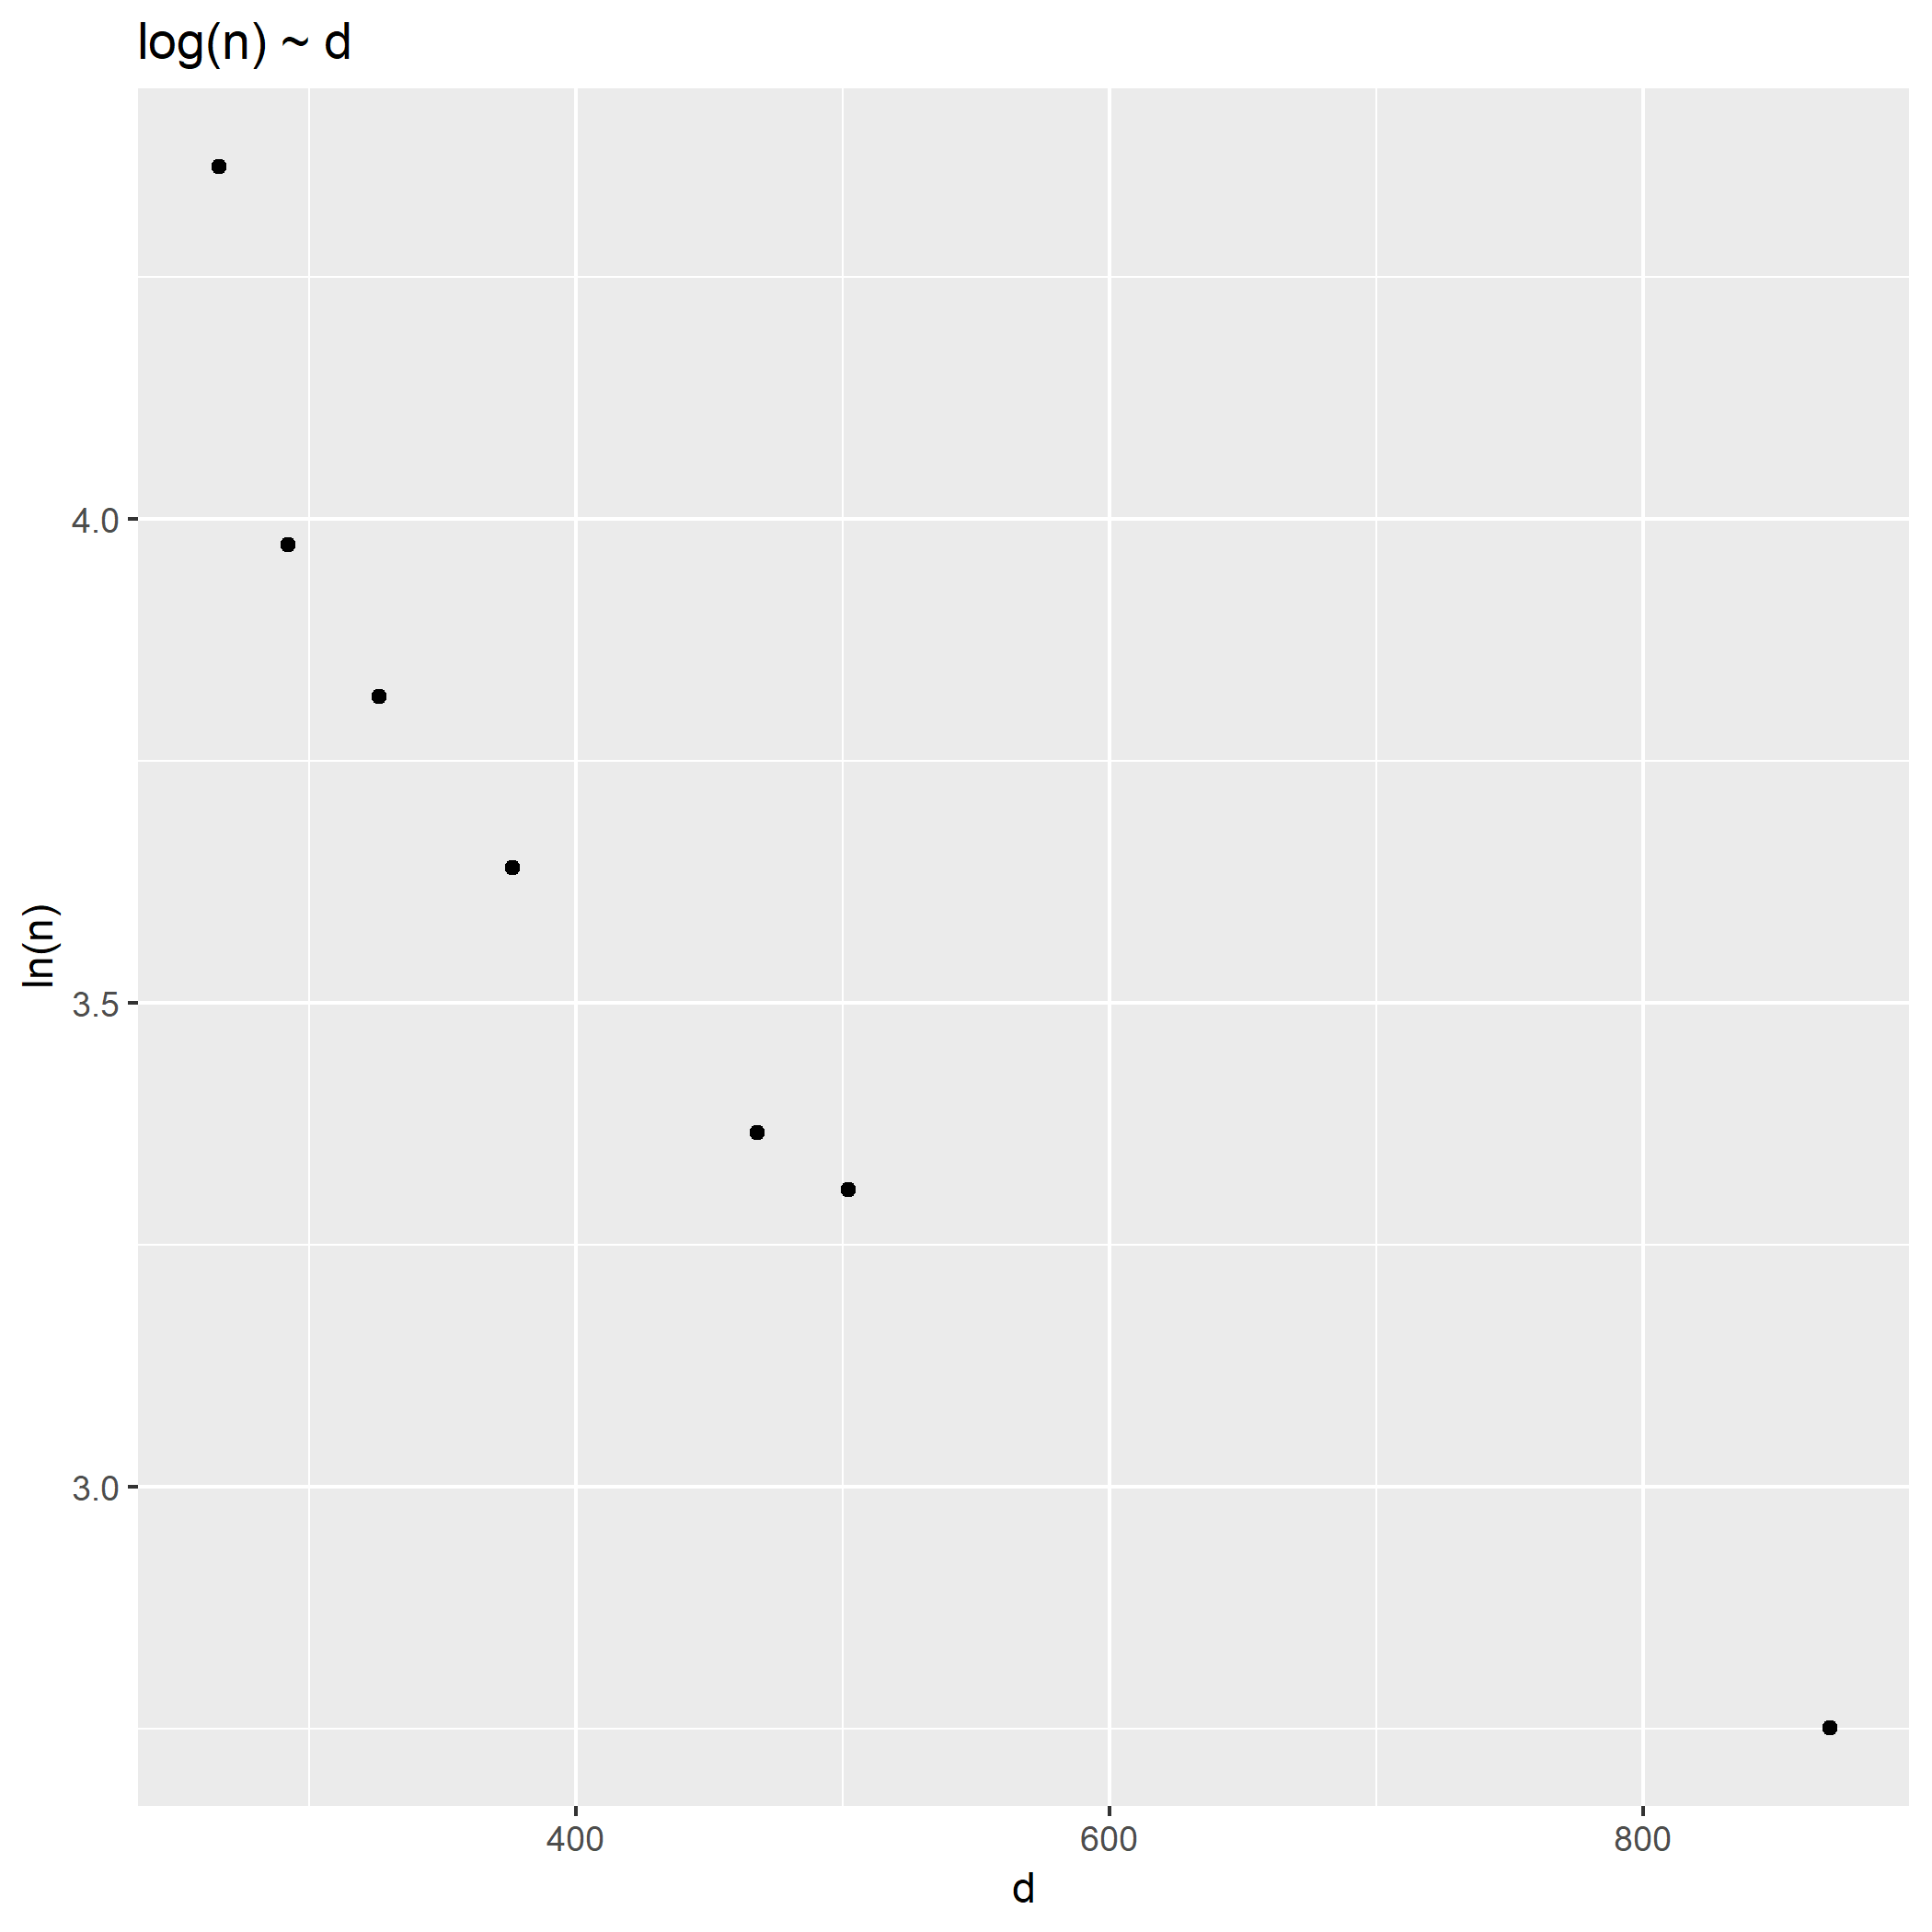
\includegraphics[width = 0.5\textwidth]{../Data/raw_point.png}
                \caption{The realtionship between distance and logarithm of number of base pairs}
                \label{raw.curve}
            \end{figure}

            After choosing some of the data points and using linear regression fitting algorithm, I derived the equation that:
            $$n = exp(4.2 - 1.7 \times 10 ^ {-3} \cdot d)$$
            where $n$ is the length (bps) of DNA fragments and $d$ is the distance these fragments travel.

            The combination of this line and data points is as follows,
            \begin{figure}[H]
                \centering
                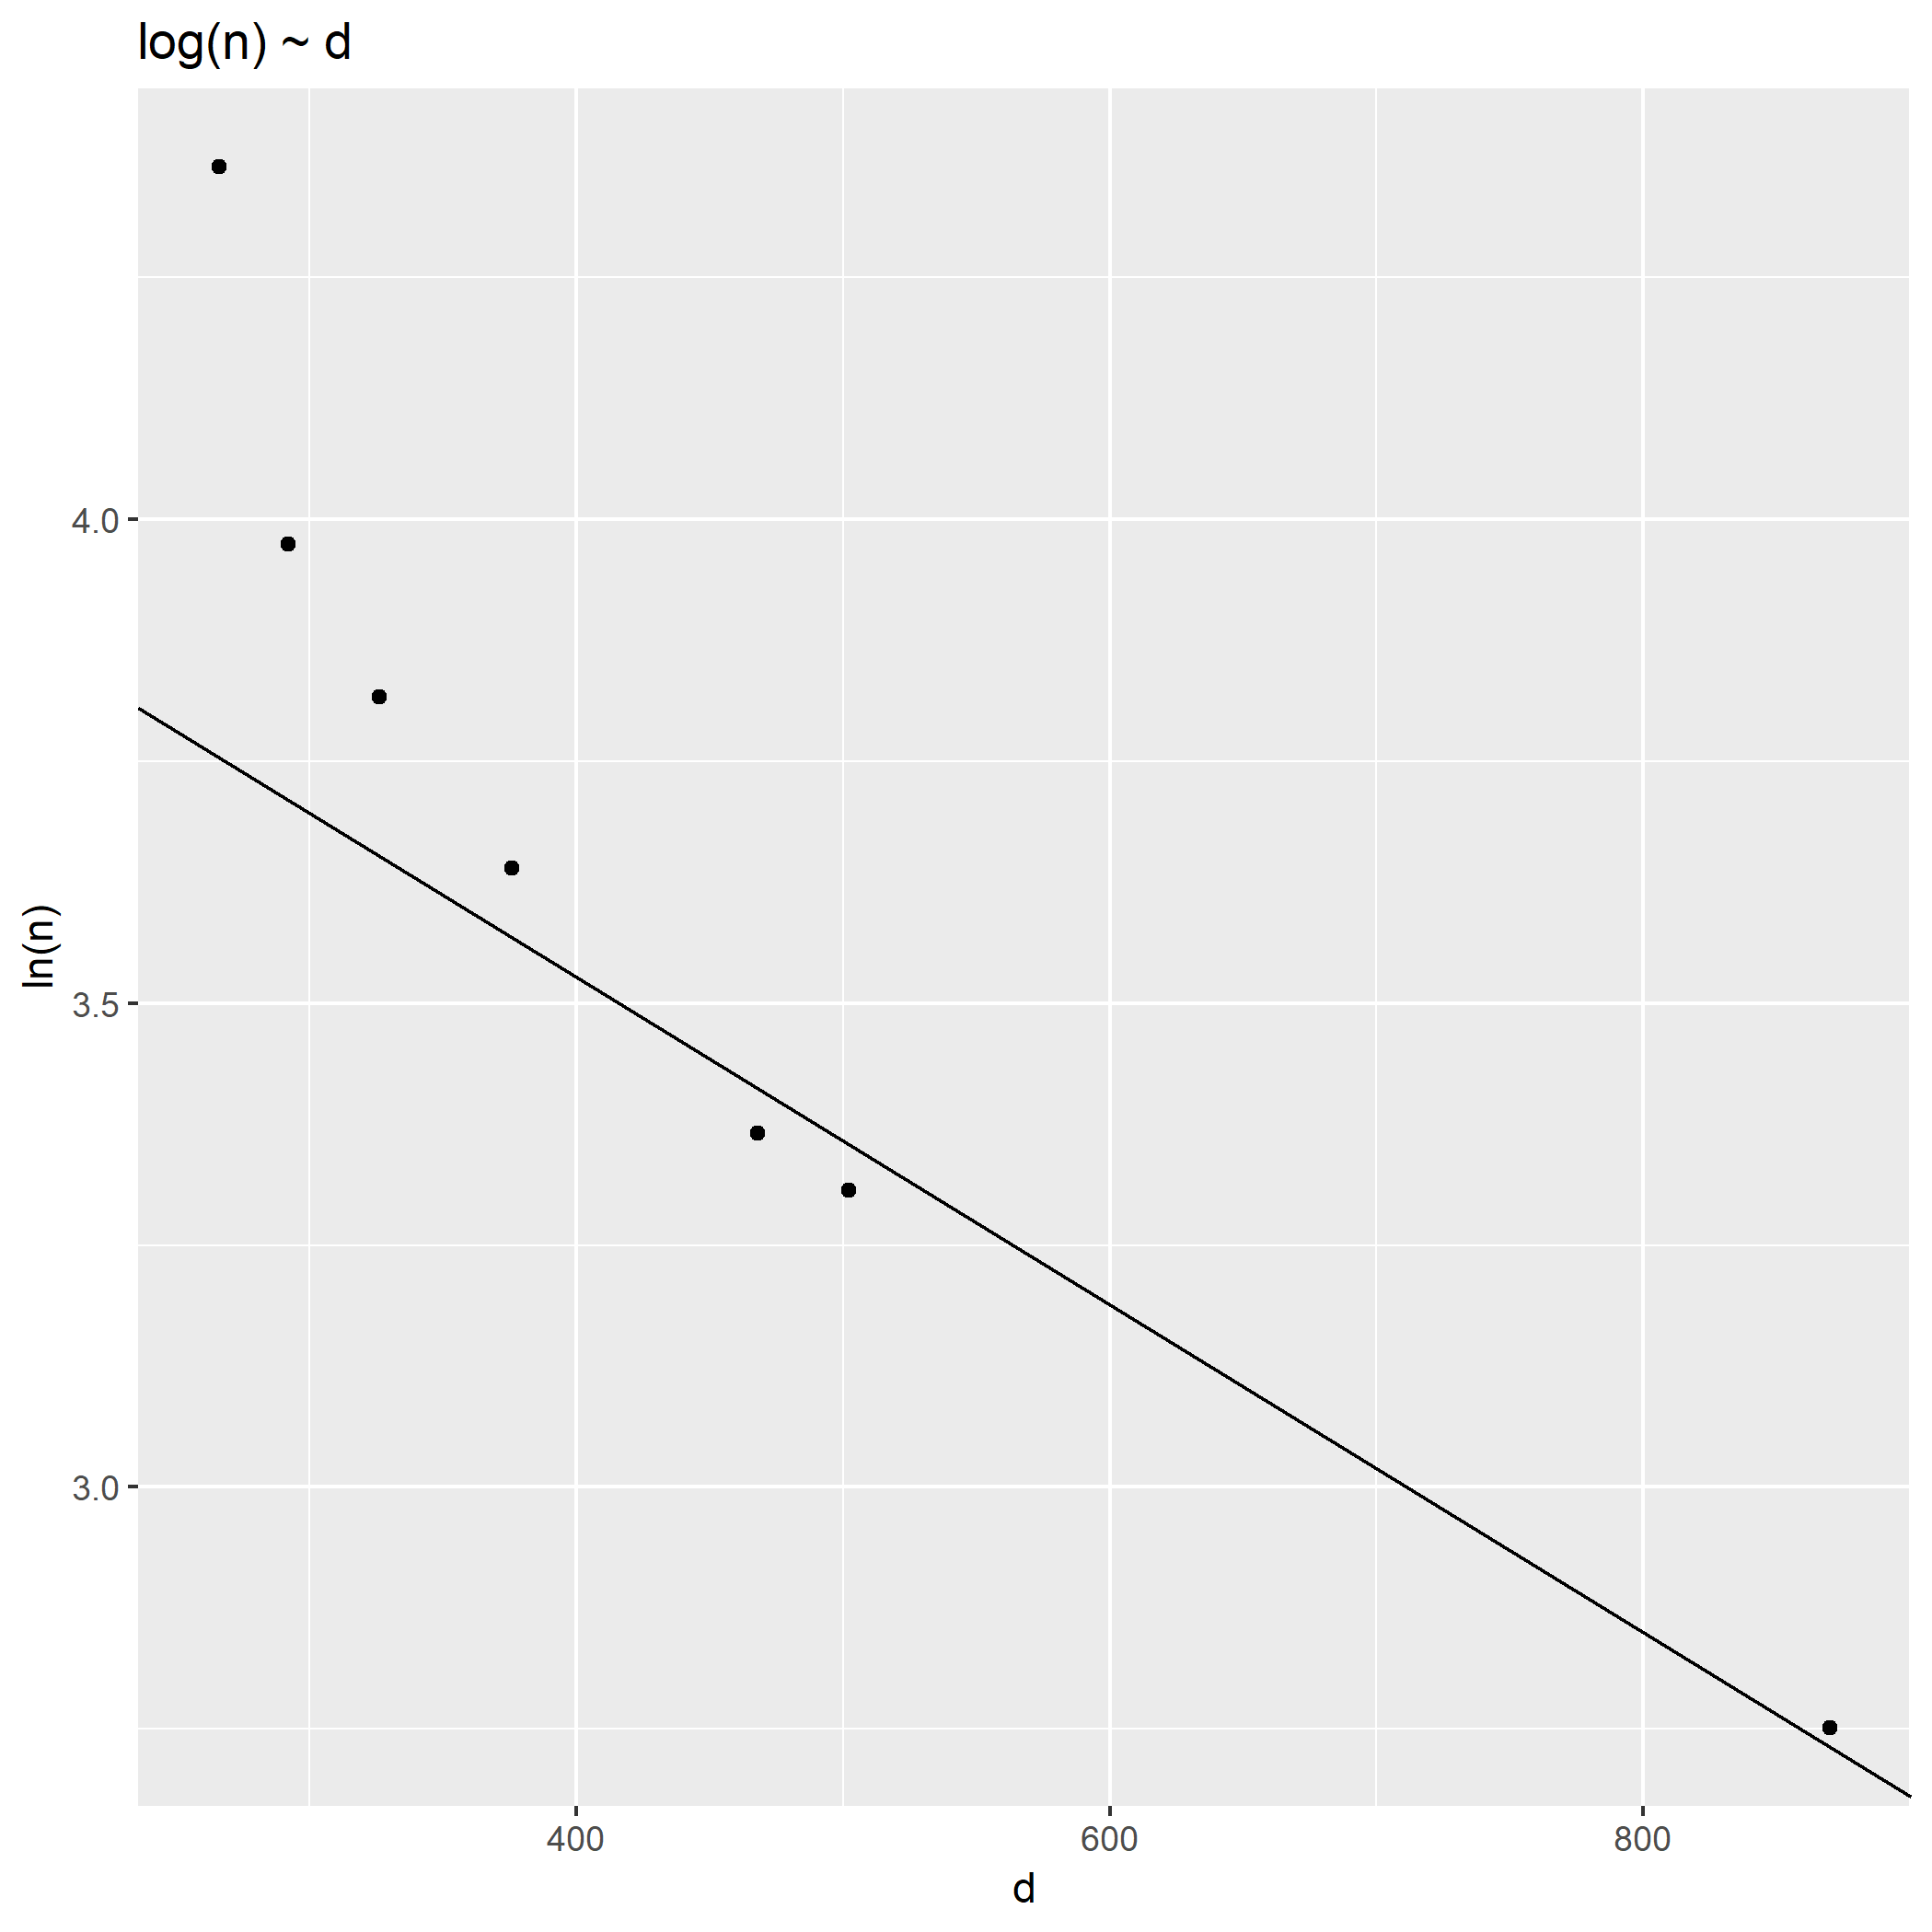
\includegraphics[width = 0.5\textwidth]{../Data/raw_points_line.png}
                \caption{Standard Curve with Fitting Line}
                \label{raw.curve.line}
            \end{figure}
            
        \subsection{pBR322 Digestion Data}
            The distance of every well is shown below, using pixel unit.
            \begin{table}[H]
                \caption{Distance}
                \begin{center}\begin{tabular}{|l|c|c|c|c|c|c|c|}
                    \hline
                    tube&E&H&P&EH&EP&HP&EHP\\
                    \hline
                    distance&400.125&418.12&388.082&424.118&472.004&520.004&530.015\\
                    (pixels)&&682.237&&676.027&486.037&596.03&602.003\\
                    &&&&830.039&&668.012&830.002\\
                    &&&&924.078&&&928.002\\
                    \hline
                \end{tabular}\end{center}
                \label{data.table}
            \end{table}
            So using the equation derived above, we can get the estimated sequence length,
            \begin{table}[H]
                \caption{Length}
                \begin{center}\begin{tabular}{|l|c|c|c|c|c|c|c|}
                    \hline
                    tube&E&H&P&EH&EP&HP&EHP\\
                    \hline
                    length&3801.894&3326.596&4149.54&3184.198&2238.721&1570.363&1458.814\\
                    (bps)&&475.335&&497.737&2018.366&897.429&859.014\\
                    &&&&159.956&&527.23&159.956\\
                    &&&&79.983&&&77.625\\
                    \hline
                \end{tabular}\end{center}
                \label{data.len.table}
            \end{table}
            and also the logarithm of length,
            \begin{table}[H]
                \caption{Logarithm of length}
                \begin{center}\begin{tabular}{|l|c|c|c|c|c|c|c|}
                    \hline
                    tube&E&H&P&EH&EP&HP&EHP\\
                    \hline
                    log(length)&3.58&3.522&3.618&3.503&3.35&3.196&3.164\\
                    &&2.677&&2.697&3.305&2.953&2.934\\
                    &&&&2.204&&2.722&2.204\\
                    &&&&1.903&&&1.89\\
                    \hline
                \end{tabular}\end{center}
                \label{data.log.table}
            \end{table}
        \subsection{pBR322 Mapping}

    
    \section{Discussion}
        \subsection{Standard Curve}
            First, I tried to discard the points with larger length, which is out of the gel's resolving ability. The lines are derived from linear regression, namely, least squared method (calculation not shown).
            \begin{figure}[H]
                \begin{minipage}[t]{0.5\textwidth}
                    \centering
                    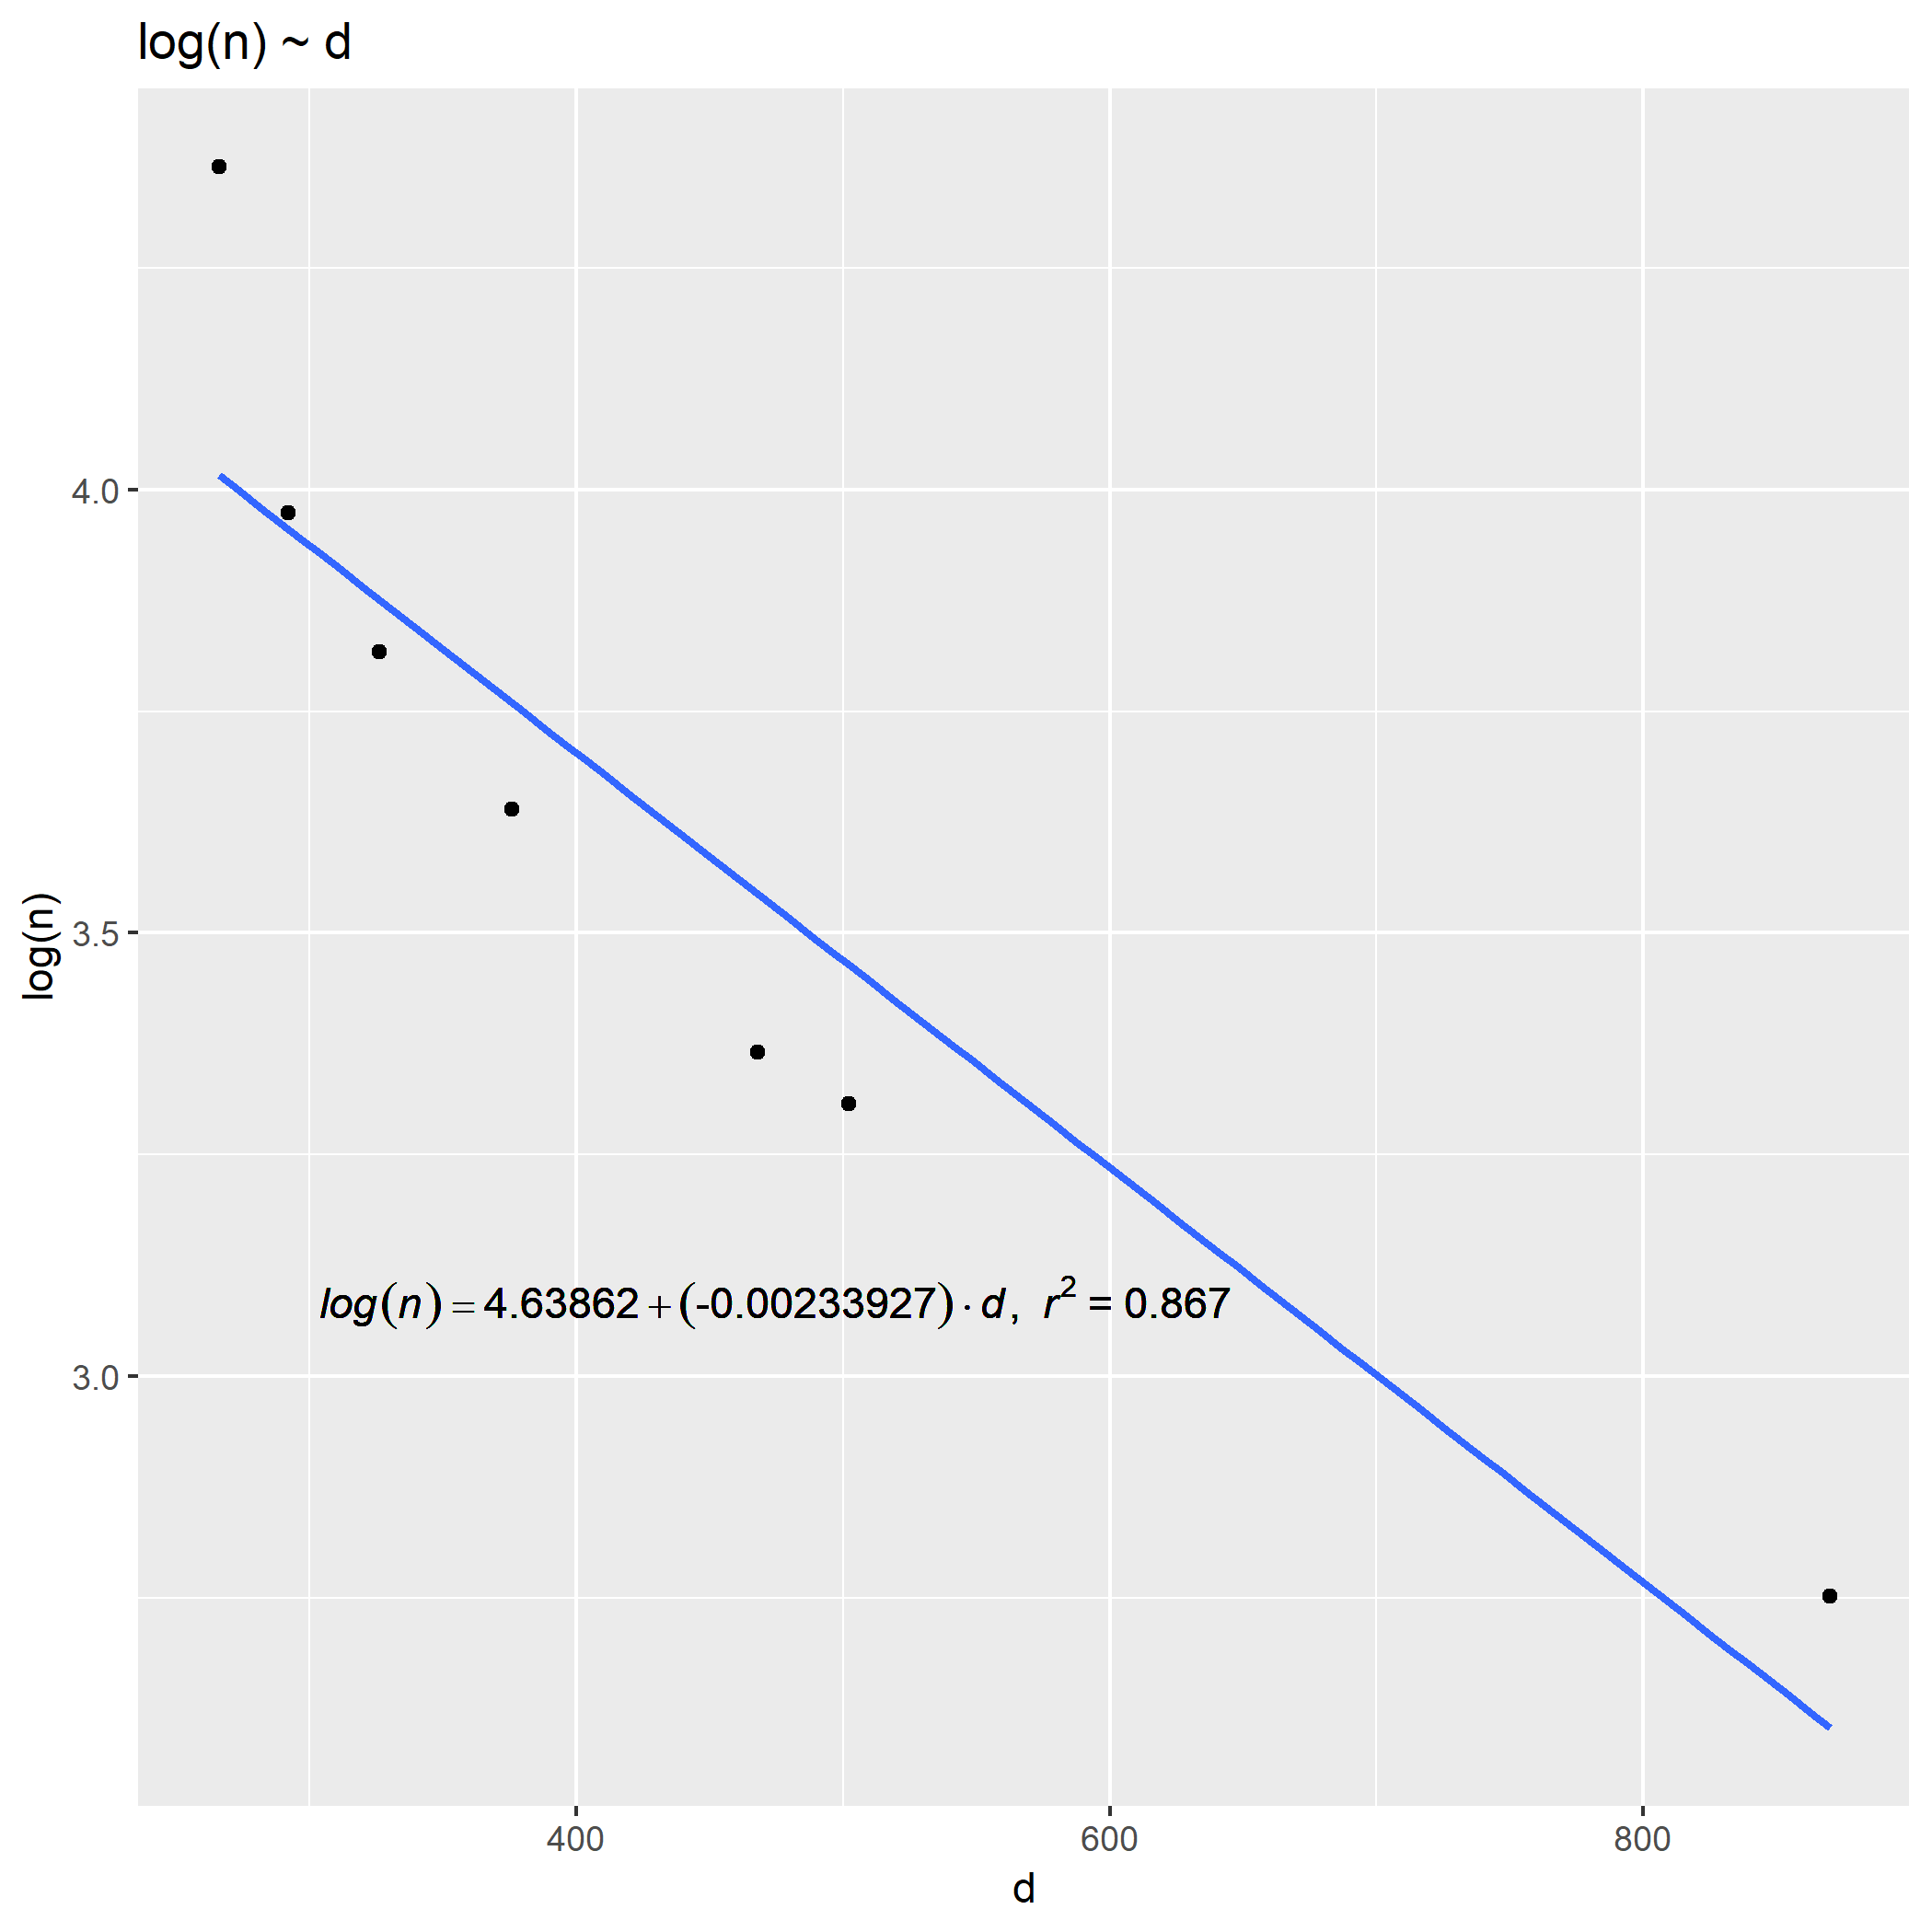
\includegraphics[width = 0.8\linewidth]{../Data/discard_1.png}
                    \caption{No Discarding}
                    \label{dis.0}
                \end{minipage}
                \begin{minipage}[t]{0.5\textwidth}
                    \centering
                    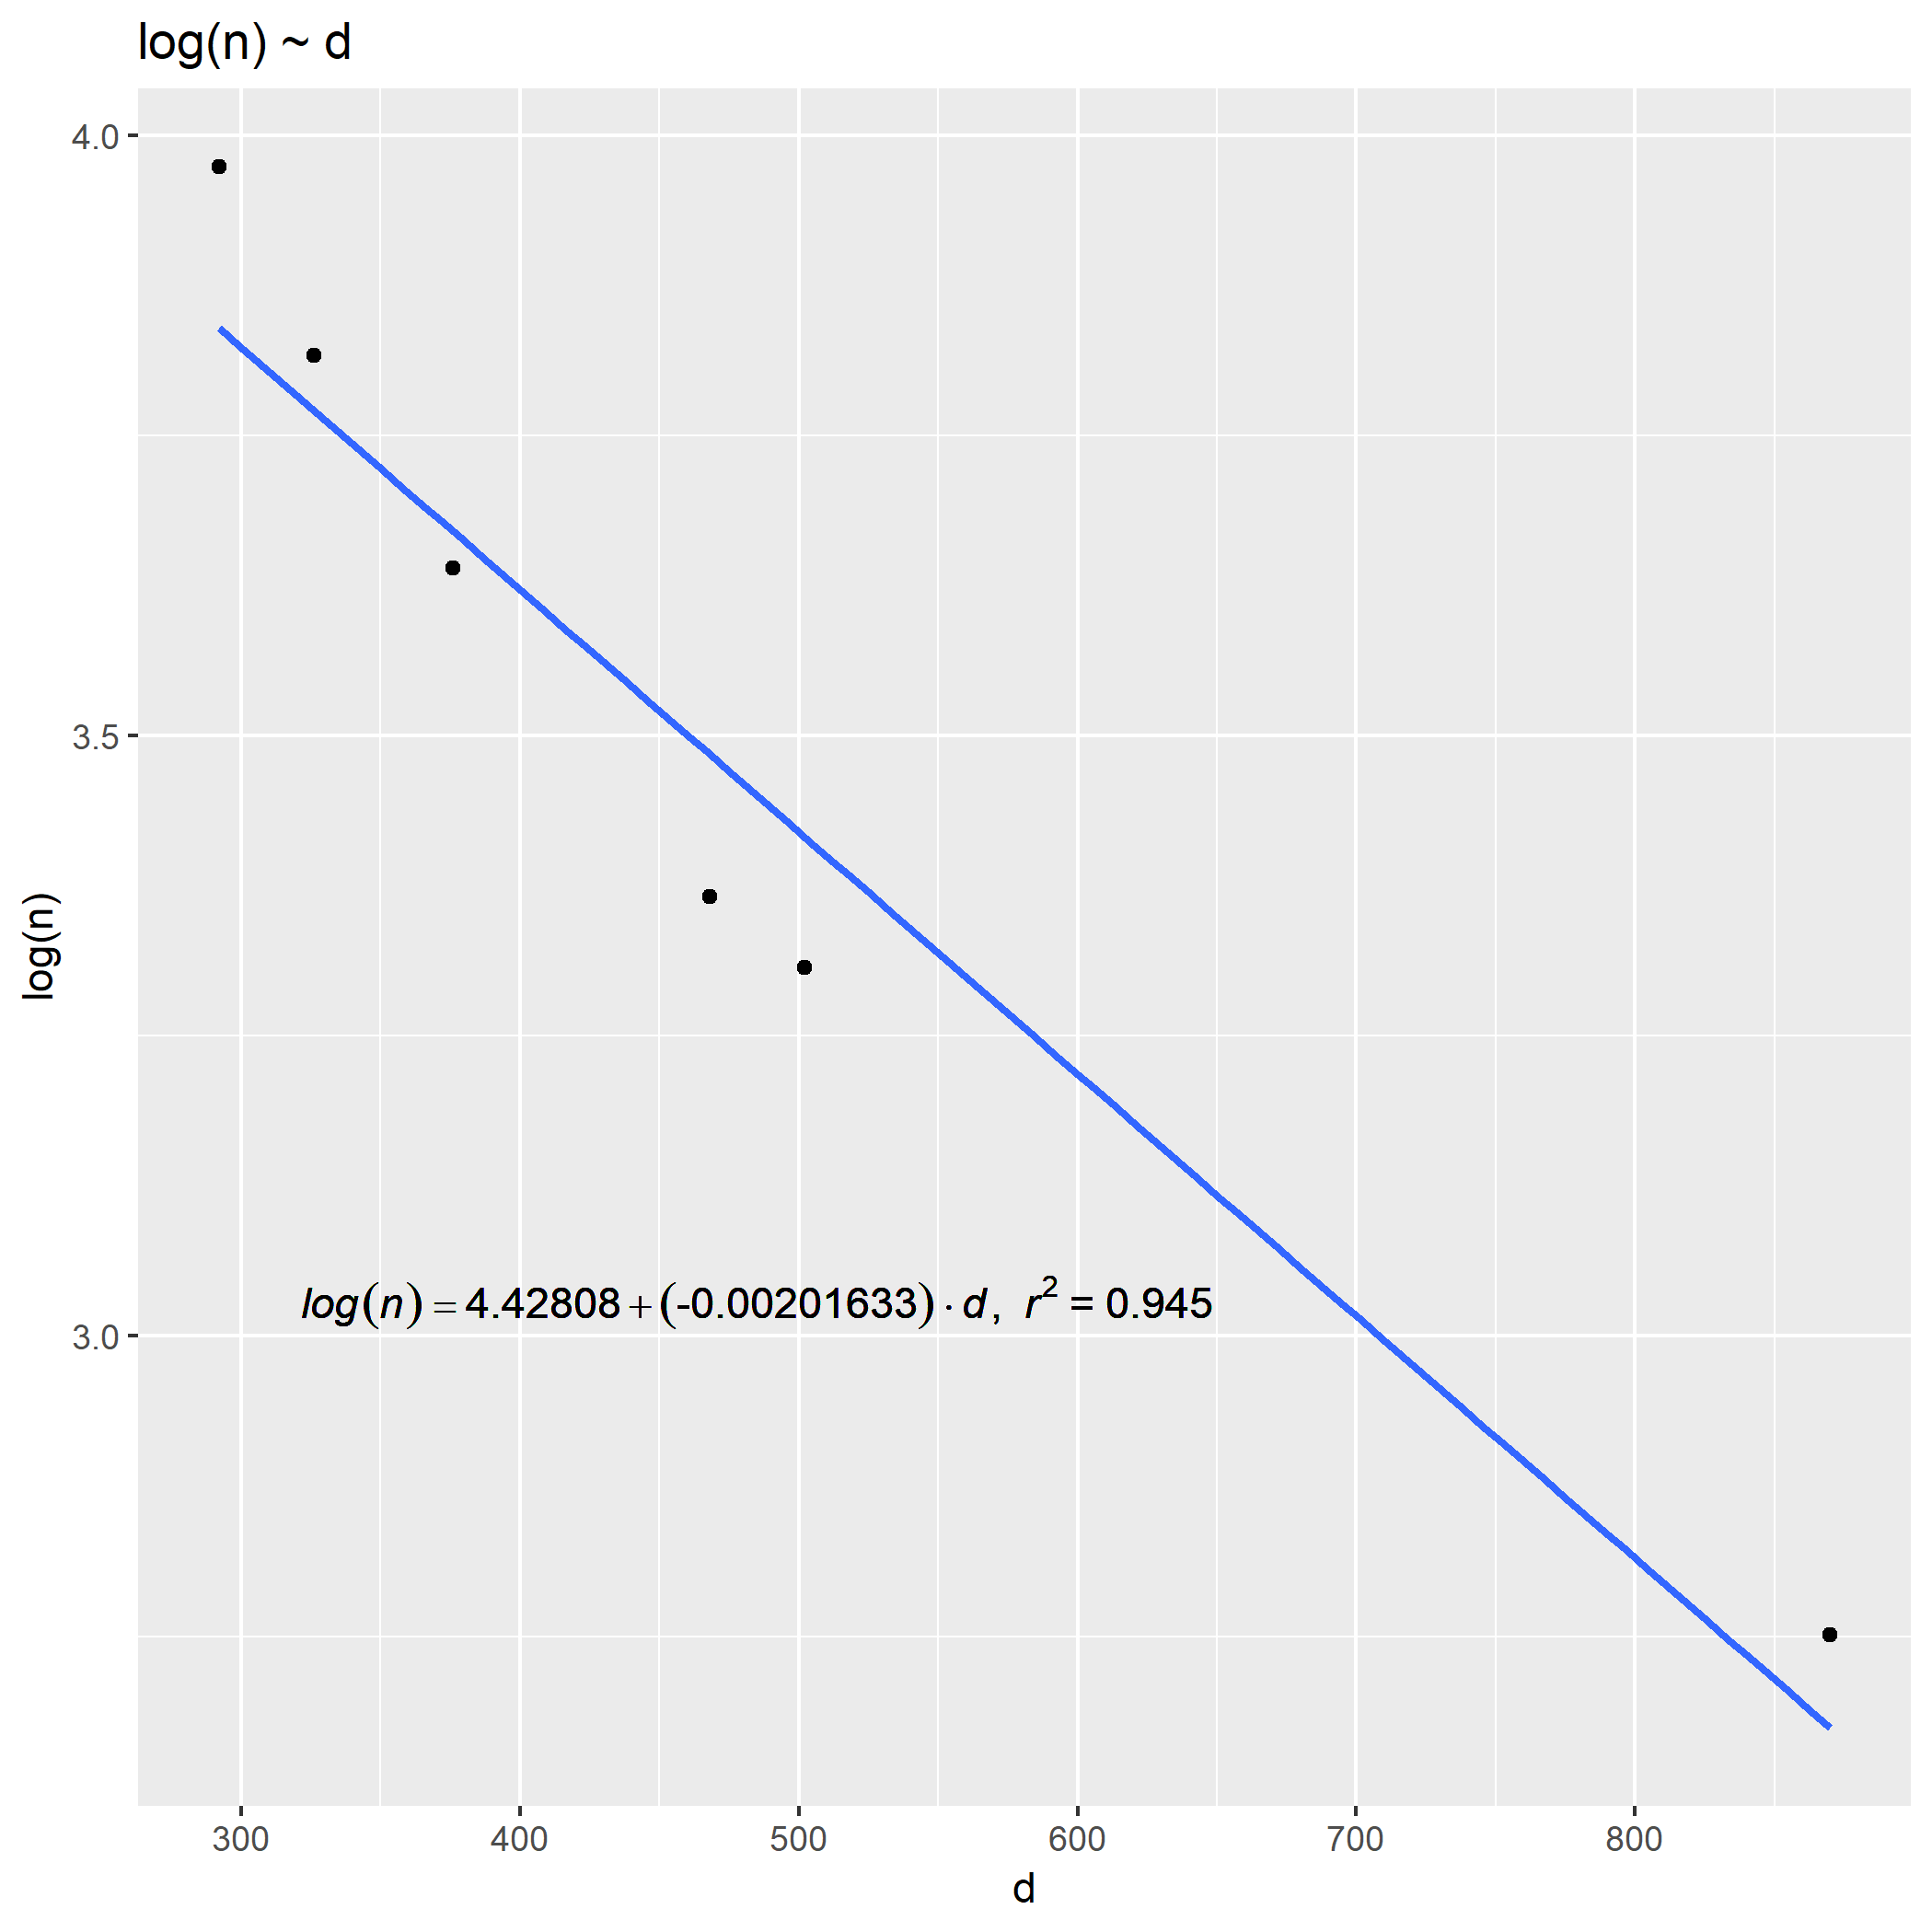
\includegraphics[width = 0.8\linewidth]{../Data/discard_2.png}
                    \caption{Discarding Point 1}
                    \label{dis.1}
                \end{minipage}
                \begin{minipage}[t]{0.5\textwidth}
                    \centering
                    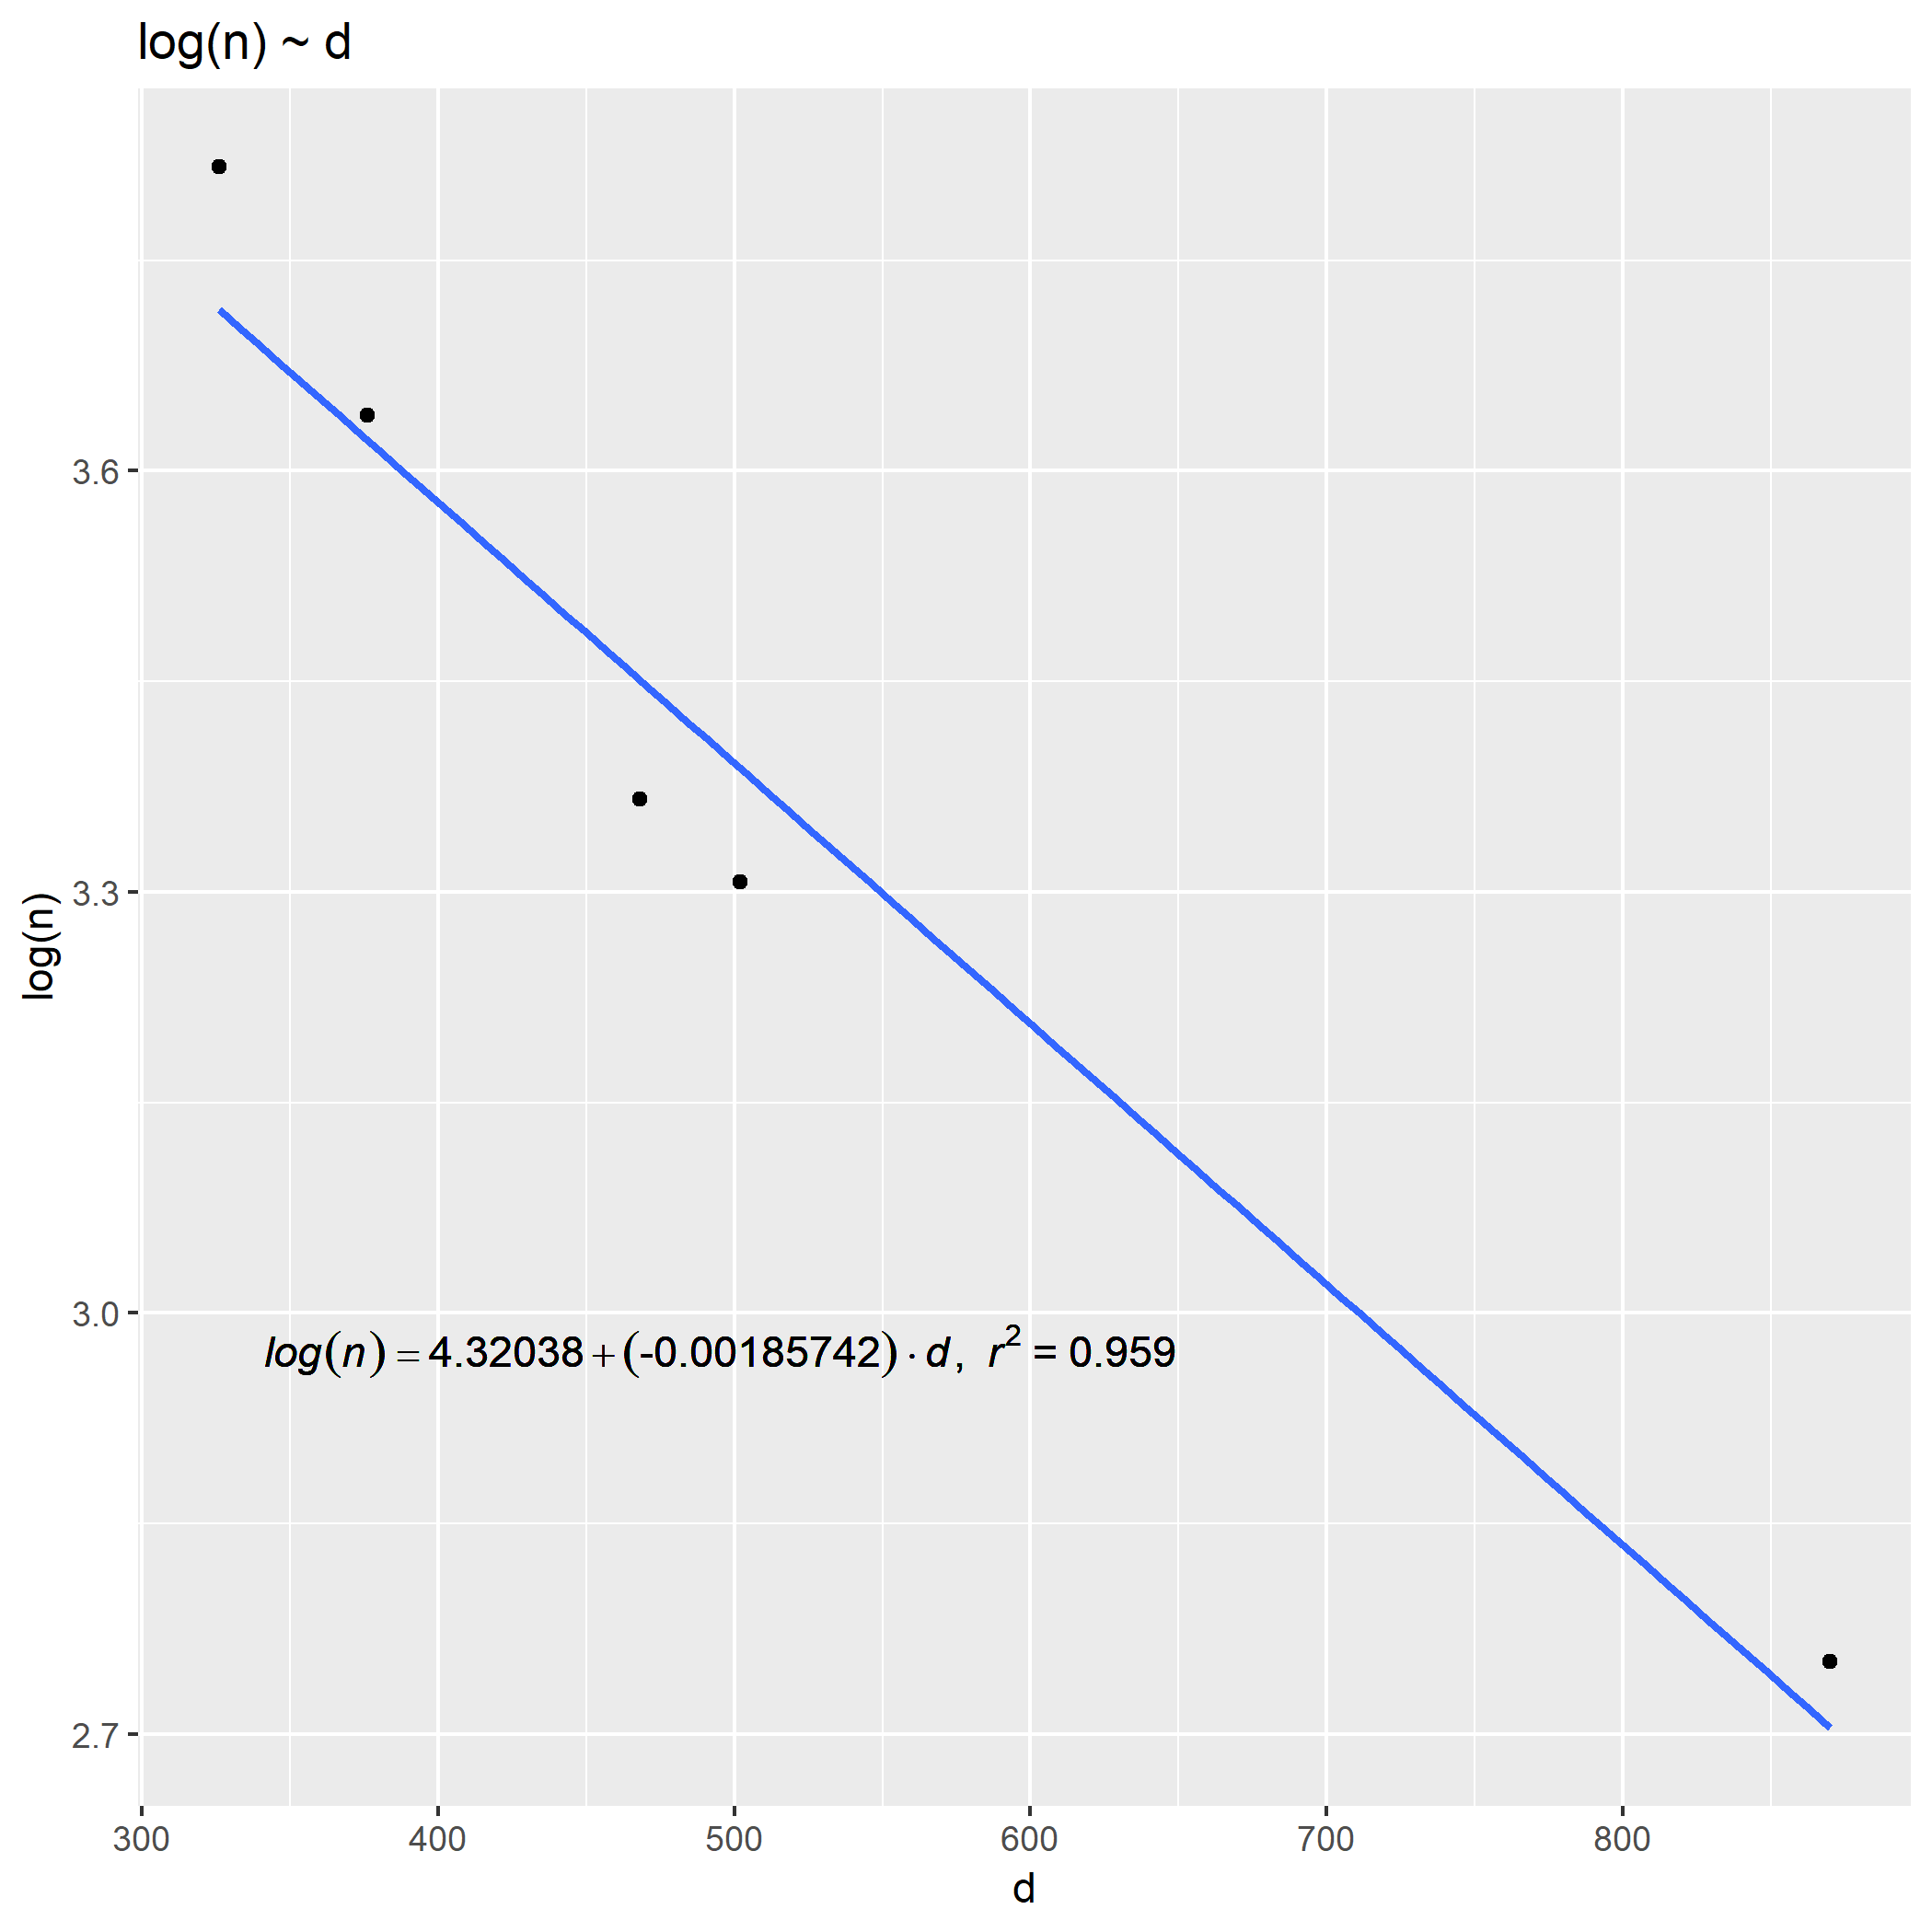
\includegraphics[width = 0.8\linewidth]{../Data/discard_3.png}
                    \caption{Discarding Point 1$\sim$2}
                    \label{dis.2}
                \end{minipage}
                \begin{minipage}[t]{0.5\textwidth}
                    \centering
                    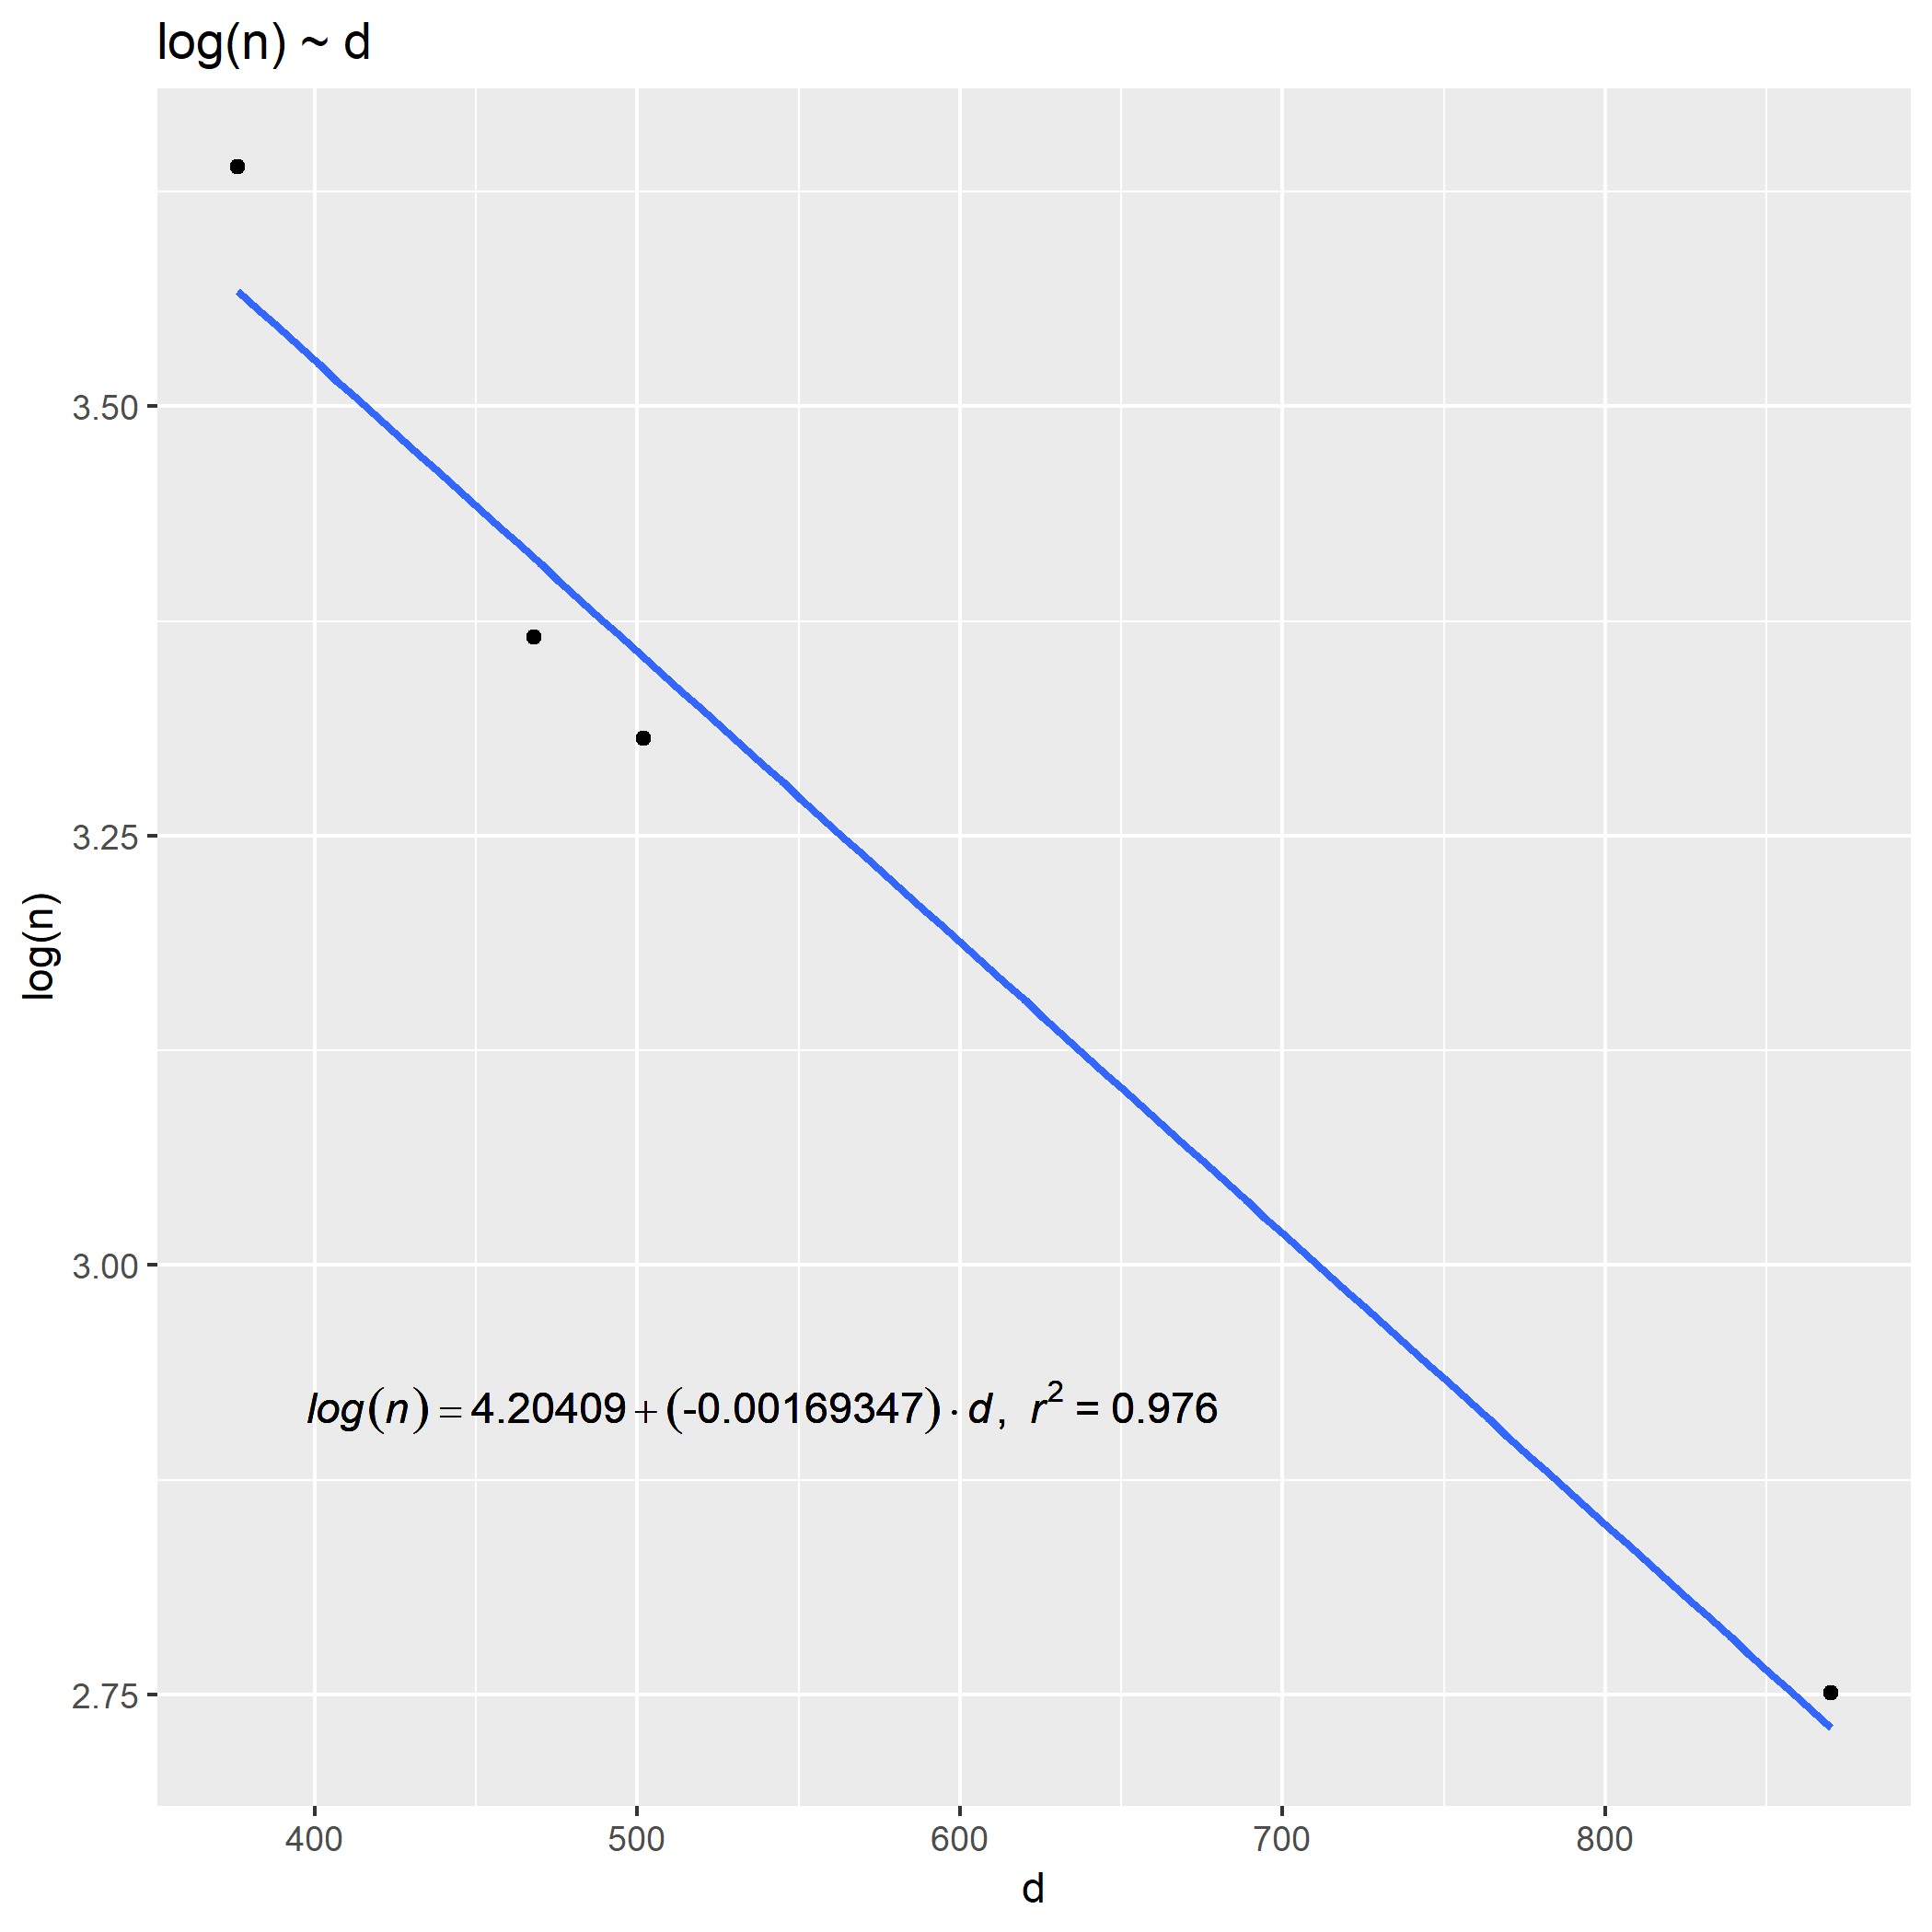
\includegraphics[width = 0.8\linewidth]{../Data/discard_4.png}
                    \caption{Discarding Point 1$\sim$3}
                    \label{dis.3}
                \end{minipage}
            \end{figure}

            Then compared the $R^2$, we can see that discarding first 3 points leads to the highest $R^2$ as $0.976$. In addition, these three points are also longer than 5000bp, larger than the ability of gel resolution. 

            If we discard more points, we would get higher $R^2$, but we will lose data information and increase the effect of random error.

            Finally we will use Figure \ref{dis.3} as the fitting line, which has already been plotted in Figure \ref{raw.curve.line} in \textbf{Result} part.

            In conclusion,
            $$
            \begin{aligned}
                \text{log}(n) &= 4.2 - 1.7\times 10 ^ {-3} \cdot d\\
                n &= exp(4.2 - 1.7 \times 10 ^ {-3} \cdot d)
            \end{aligned}
            $$

        \subsection{Relative Position Analysis}
            For convenience, I label bands from tube \textbf{E, H, P, EH, EP, HP, EHP}.
            \begin{figure}[H]
                \centering
                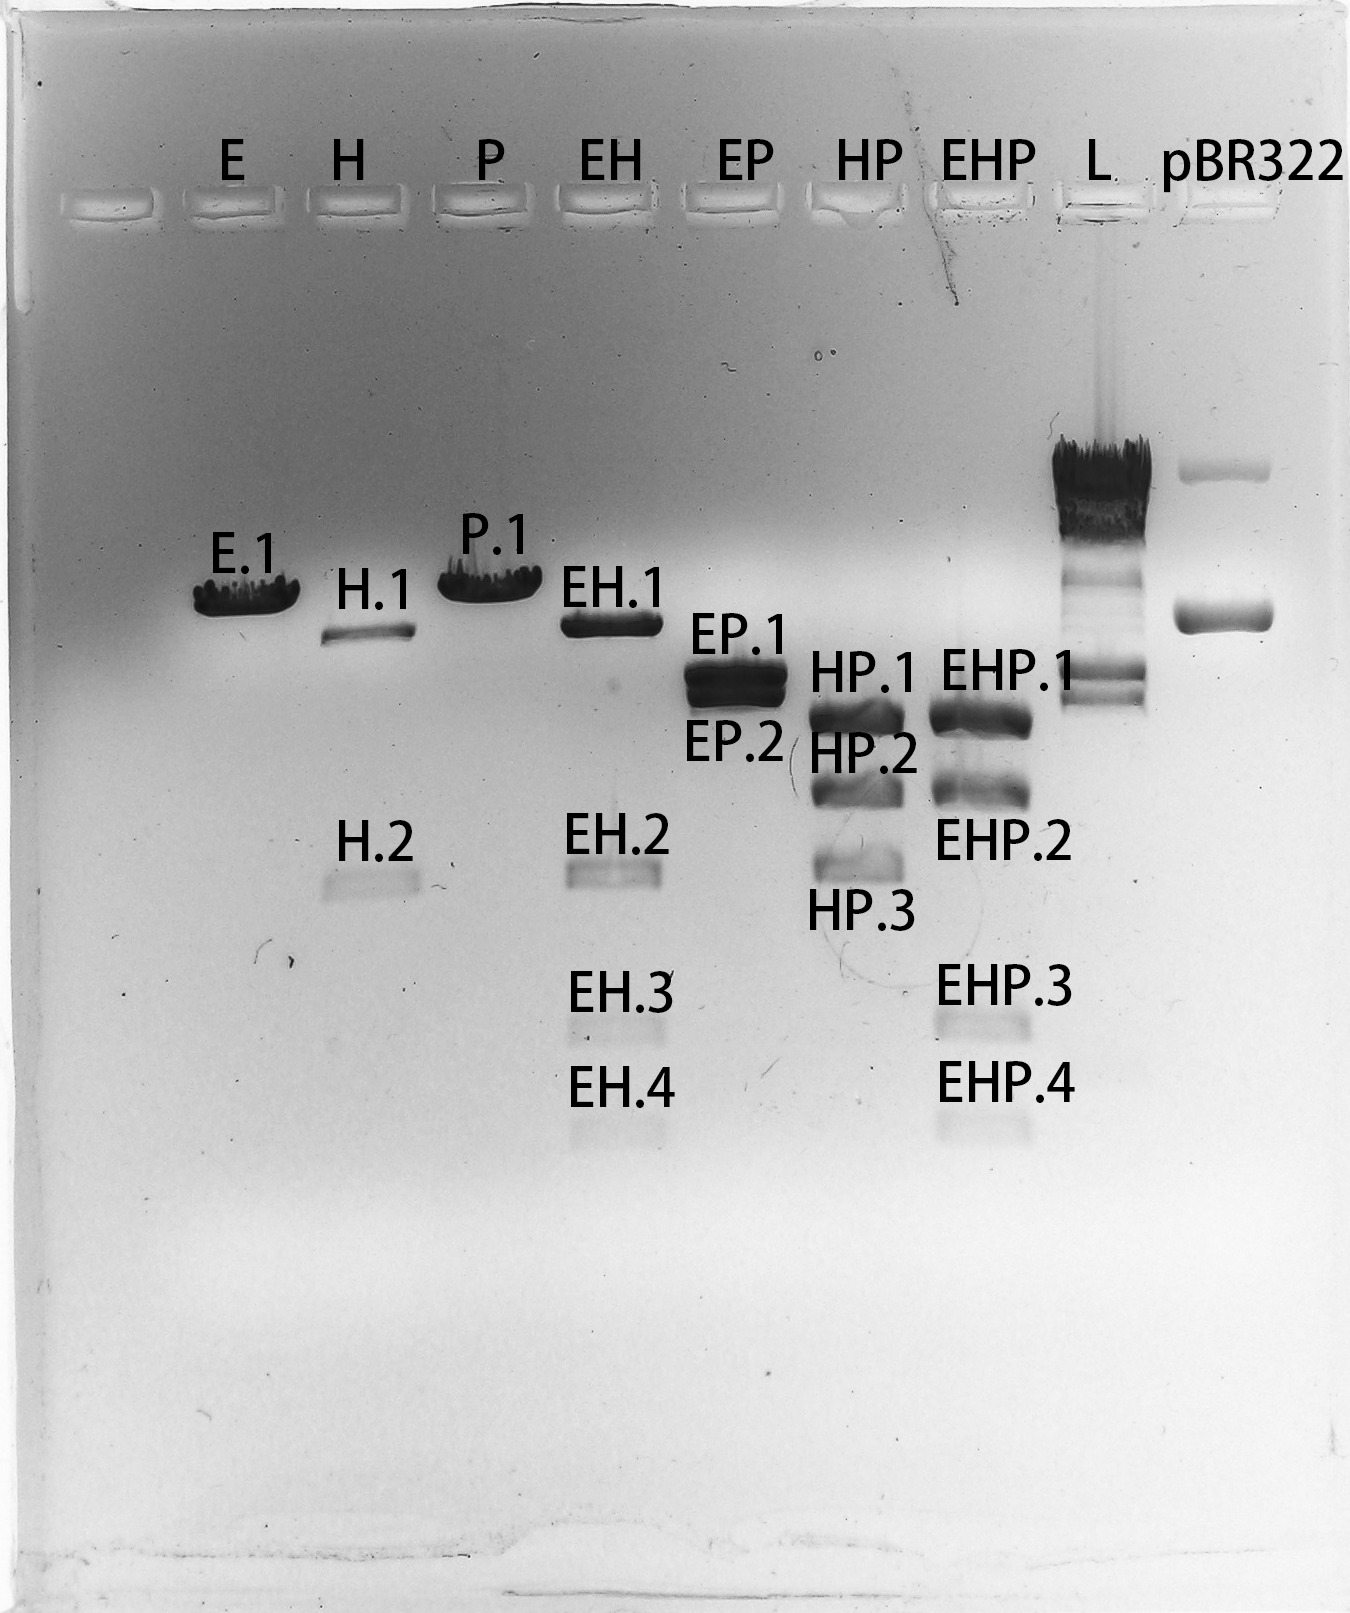
\includegraphics[width = 0.5\linewidth]{../Data/xun_and_sam_label.png}
                \caption{Labeled Bands}
                \label{label.bands}
            \end{figure}
\end{document}